% ==============================================================================
% 第 33 章：累加器的更多应用 (Chapter 33: More Uses of Accumulation)
% ==============================================================================

\chapter{累加器的更多应用}
\label{sec:ch33_more_uses}

本章展示累加器的三种进阶应用场景。第一节探讨累加器在树形数据结构处理函数中的关键应用，以 ISL+ 编译器的语法分析与变量作用域检查为例展开剖析。第二节解释为什么有时需要将累加器直接嵌入到数据表示结构之中（即\term{数据累加器}），并通过经典博弈谜题展示其不可替代的价值。最后一节回到分形图形的递归绘制，阐述累加器作为函数计算结果的独特运作模式。

\section{累加器与树}
\label{sec:ch33_1}

当你在 DrRacket 中点击运行一个 ISL+ 程序时，DrRacket 会将你的源代码转译为底层物理计算机能够执行的机器指令。这一过程被称为\term{编译}（compilation），而负责执行该任务的核心组件称为\term{编译器}（compiler）。在编译器对 ISL+ 程序进行底层翻译之前，它首先必须严格检查程序中的每一个变量是否已经通过 \code{define}、\code{define-struct} 或 \code{lambda} 进行了合法声明。

\begin{notebox}[请停下来在 DrRacket 中验证！]
尝试在 DrRacket 定义区中分别输入 \code{x}、\code{(lambda (y) x)} 以及 \code{(x 5)} 作为完整的 ISL+ 程序并点击运行。你预期会观察到什么现象？
\end{notebox}

让我们将上述编译器语法分析任务提炼为一个具有代表性的范例问题：

\begin{notebox}[问题陈述：迷你语言编译器与未声明变量检查]
你受聘参与复现 ISL+ 编译器的一部分核心功能。具体而言，你的任务是处理由以下文法规则（许多编程语言规范所通用的语法表示法）所定义的迷你语言片段：
\begin{lstlisting}[language=BSL]
; 文法表示：
;   λ-expr = Variable
;          | (λ (Variable) λ-expr)
;          | (λ-expr λ-expr)
\end{lstlisting}
\begin{notebox}[记号说明]
我们使用希腊字母 $\lambda$ 代替关键字 \code{lambda}，以强调此时我们是将 ISL+ 作为\textbf{被研究的客体语言}，而不仅仅作为编写代码的工具。
\end{notebox}
请回忆插曲 1 中的规则：在阅读此类文法时，可以将等号 \code{=} 朗读为“是下列之一”，将竖线 \code{|} 朗读为“或者”。

回忆 $\lambda$ 表达式表示匿名函数。它们在其函数体内部\term{绑定}（bind）其形式参数；反之，程序中某个变量的出现，由外层包裹它的、具有相同形参名称的最近一个 $\lambda$ 进行声明。

请为上述语言片段设计数据表示（使用符号表示变量名）；然后设计一个函数，将所有未声明的自由变量替换为特定的错误标识符 \code{\textquotesingle *undeclared}。
\end{notebox}

在深入算法设计之前，让我们重温基于 $\lambda$ 表达式构建的若干典型示例：
\begin{itemize}
  \item \code{($\lambda$ (x) x)}：接收什么就返回什么的恒等函数（identity function）；
  \item \code{($\lambda$ (x) y)}：试图接收参数并返回 \code{y}，但其中的 \code{y} 根本未被声明；
  \item \code{($\lambda$ (y) ($\lambda$ (x) y))}：高阶柯里化函数，接收值 $v$ 后返回一个始终产生 $v$ 的常数函数；
  \item \code{(($\lambda$ (x) x) ($\lambda$ (x) x))}：将恒等函数应用于恒等函数自身；
  \item \code{(($\lambda$ (x) (x x)) ($\lambda$ (x) (x x)))}：著名的自复制无休止死循环表达式；
  \item \code{((($\lambda$ (y) ($\lambda$ (x) y)) ($\lambda$ (z) z)) ($\lambda$ (w) w))}：复合函数应用。
\end{itemize}

\begin{exercise}{分析迷你语言中的变量作用域}{511}
分析上述各个示例中每个形参绑定的\term{作用域}（scope）。在草稿纸上绘制指向箭头，从每个被绑定的变量出现处指向其外层对应的 $\lambda$ 绑定声明处。
\end{exercise}

为该语言设计数据表示非常自然，我们将其命名为 \code{Lam}：

\begin{lstlisting}[language=BSL]
; A Lam is one of:
; -- a Symbol
; -- (list 'λ (list Symbol) Lam)
; -- (list Lam Lam)

(define ex1 '(λ (x) x))
(define ex2 '(λ (x) y))
(define ex3 '(λ (y) (λ (x) y)))
(define ex4 '((λ (x) (x x)) (λ (x) (x x))))
\end{lstlisting}

\begin{exercise}{定义语法谓词与选择器}{512}
为 \code{Lam} 定义判定谓词 \code{is-var?}、\code{is-lambda?} 与 \code{is-app?}，分别用于识别变量、$\lambda$ 抽象与函数应用。

同时定义提取组件的选择器函数：
\begin{enumerate}
  \item \code{$\lambda$-para}：从 $\lambda$ 表达式中提取形参符号；
  \item \code{$\lambda$-body}：从 $\lambda$ 表达式中提取函数体表达式；
  \item \code{app-fun}：从函数应用中提取操作符函数项；
  \item \code{app-arg}：从函数应用中提取操作数实参项。
\end{enumerate}
此外，设计函数 \code{declareds}，提取给定 \code{Lam} 项中用作 $\lambda$ 形参的所有符号列表。
\end{exercise}

\begin{exercise}{为迷你语言设计基于结构体的数据表示}{513}
利用 \code{define-struct} 为上述 ISL+ 语言子集设计基于结构体的数据表示替代方案，并使用新结构体实例化表示 \code{ex1}、\code{ex2} 与 \code{ex3}。
\end{exercise}

现在，让我们针对未声明变量检测函数 \code{undeclareds} 进行设计：

\begin{lstlisting}[language=BSL]
; Lam -> Lam
; 将 le0 中所有未在任何外层绑定 λ 形参作用域内的变量替换为 '*undeclared
(check-expect (undeclareds ex1) ex1)
(check-expect (undeclareds ex2) '(λ (x) *undeclared))
(check-expect (undeclareds ex3) ex3)
(check-expect (undeclareds ex4) ex4)
(define (undeclareds le0)
  le0)
\end{lstlisting}

审视该函数的目的说明，我们立即发现：\textbf{常规的结构型递归在深入 $\lambda$ 函数体时，会不可避免地遗忘外层所声明的形参！}这一知识丢失在模板中暴露无遗：

\begin{lstlisting}[language=BSL]
(define (undeclareds le)
  (cond
    [(is-var? le) ...]
    [(is-λ? le)
     (... (λ-para le) ...
      ... (undeclareds (λ-body le)) ...)]
    [(is-app? le)
     (... (undeclareds (app-fun le)) ...
      ... (undeclareds (app-arg le)) ...)]))
\end{lstlisting}

当函数递归进入 \code{($\lambda$-body le)} 时，形参 \code{($\lambda$-para le)} 就在当前上下文中消失了。这强烈提示我们必须引入累加器：

\begin{lstlisting}[language=BSL]
(define (undeclareds.v2 le0)
  (local (
    (define (undeclareds/a le a)
      (cond
        [(is-var? le) ...]
        [(is-λ? le)
         (... (λ-para le) ...
          ... (undeclareds/a (λ-body le) (... a ...)) ...)]
        [(is-app? le)
         (... (undeclareds/a (app-fun le) a) ...
          ... (undeclareds/a (app-arg le) a) ...)])))
    (undeclareds/a le0 '())))
\end{lstlisting}

由此，我们得出严密的累加器不变量：
\begin{quote}
\textit{累加器 \code{a}（或命名为 \code{declareds}）代表从语法树根节点 \code{le0} 到当前子表达式节点 \code{le} 的祖先路径上，所遇到的全部 $\lambda$ 形参符号的列表。}
\end{quote}

图 \ref{fig:186} 将 \code{Lam} 表达式描绘为一棵倒立的语法树（根在顶部，\code{@} 节点表示函数应用）。粗线路径清晰展示了从根节点到某子树所经过的变量声明节点。

\begin{figure}[htbp]
  \centering
  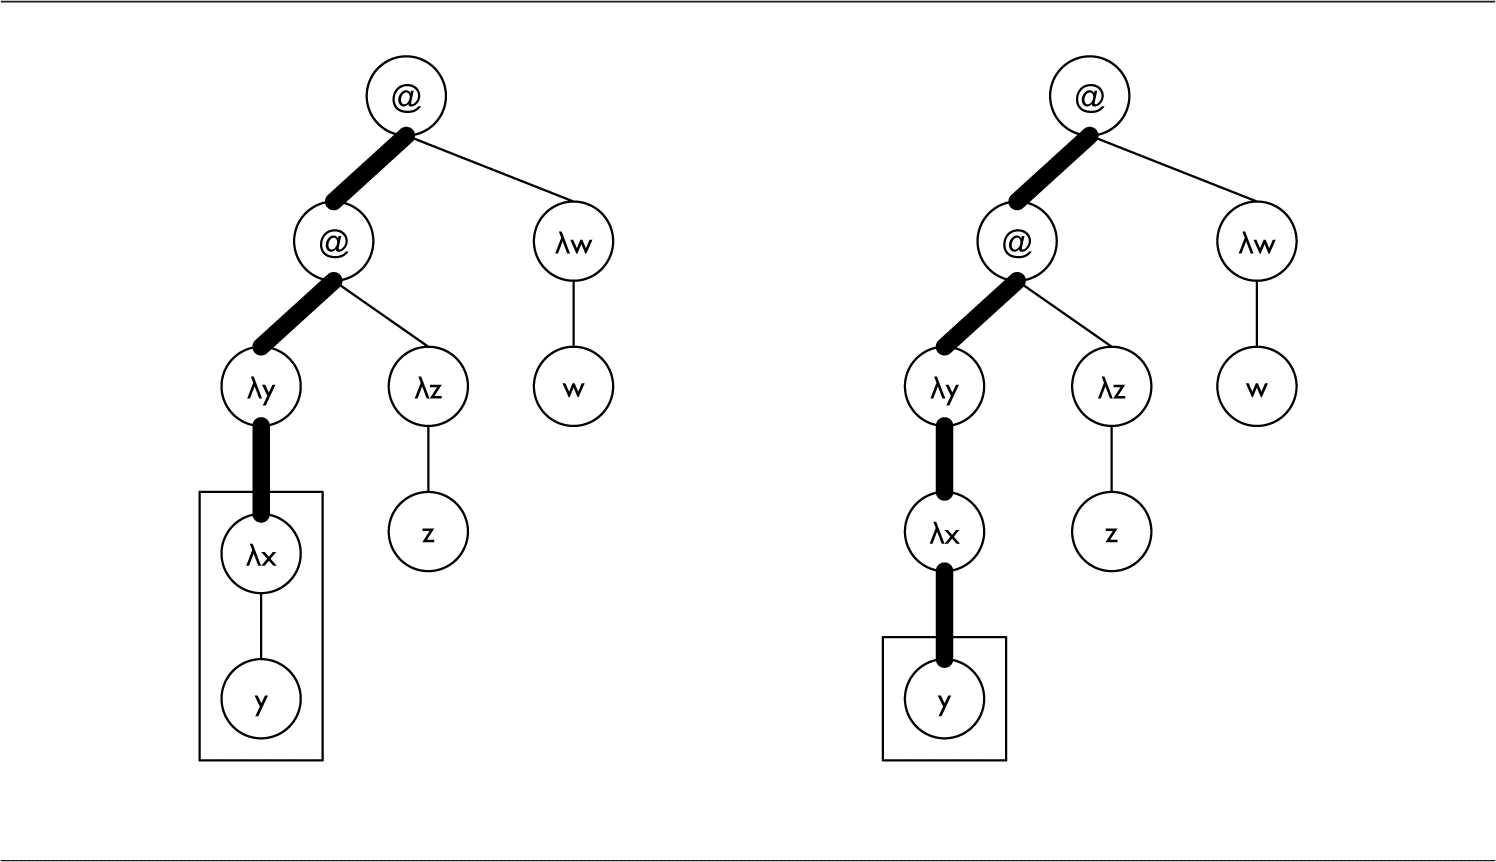
\includegraphics[width=0.85\textwidth]{images/00763.png}
  \caption{将 Lam 语法项表示为抽象语法树及其祖先声明路径}
  \label{fig:186}
\end{figure}

基于这一不变量，算法的各个组成部分彻底确立：
\begin{itemize}
  \item 初始值：从根节点出发时尚未遇到任何形参，初始为 \code{\textquotesingle()}；
  \item 更新规则：当穿越 $\lambda$ 节点深入函数体时，将新形参加入累加器：\code{(cons ($\lambda$-para le) declareds)}；
  \item 基准条件（变量节点）：利用累加器中保存的知识，调用 \code{(member? le declareds)} 检查当前变量是否在已声明列表中。若不在，替换为 \code{\textquotesingle *undeclared}；若在，保持原变量名不变。
\end{itemize}

图 \ref{fig:187} 给出了完整的实现代码。

\begin{figure}[htbp]
  \centering
\begin{lstlisting}[language=BSL, basicstyle=\scriptsize\ttfamily]
; Lam -> Lam
(define (undeclareds le0)
  (local (; Lam [List-of Symbol] -> Lam
          ; accumulator declareds is a list of all λ
          ; parameters on the path from le0 to le
          (define (undeclareds/a le declareds)
            (cond
              [(is-var? le)
               (if (member? le declareds) le '*undeclared)]
              [(is-λ? le)
               (local ((define para (λ-para le))
                       (define body (λ-body le))
                       (define newd (cons para declareds)))
                 (list 'λ (list para)
                       (undeclareds/a body newd)))]
              [(is-app? le)
               (local ((define fun (app-fun le))
                       (define arg (app-arg le)))
                 (list (undeclareds/a fun declareds)
                       (undeclareds/a arg declareds)))])))
    (undeclareds/a le0 '())))
\end{lstlisting}
  \caption{使用累加器在抽象语法树中查找并替换未声明变量}
  \label{fig:187}
\end{figure}

\begin{exercise}{自由变量与绑定变量同存的复杂项测试}{514}
构造一个同一个变量名 \code{x} 既作为自由变量出现、又在局部子项中作为绑定变量出现的 ISL+ 表达式，并用 \code{Lam} 结构表示。验证 \code{undeclareds} 在该表达式上是否能够精确区分并产生符合预期的正确结果。
\end{exercise}

\begin{exercise}{在语法树中高亮区分绑定状态}{515}
修改 \code{undeclareds}，使得当遇到未声明的自由变量 \code{\textquotesingle x} 时，将其替换为 \code{(list \textquotesingle *undeclared \textquotesingle x)}；而当遇到已正确声明的绑定变量 \code{\textquotesingle y} 时，将其替换为 \code{(list \textquotesingle *declared \textquotesingle y)}。这种精细标注正是现代 IDE（如 DrRacket）在语法检查阶段高亮着色不同变量的核心基础。
\end{exercise}

\begin{exercise}{针对结构体表示重构语法分析器}{516}
针对练习 \ref{ex:513} 中基于结构体定义的抽象语法树表示，重新实现 \code{undeclareds} 函数。
\end{exercise}

\begin{exercise}{静态距离与 De Bruijn 索引设计}{517}
设计函数 \code{static-distance}。该函数将变量名替换为一个自然数，表示其距离声明它的那个 $\lambda$ 节点向树根方向跨越的步数（计算机科学中著名的 \term{De Bruijn 索引}）。图 \ref{fig:188} 形象展示了这一转换：原树中的变量被无名 $\lambda$ 与向上层级步数所取代（0 表示直接外层的 $\lambda$，1 表示再向上一层，依此类推）。

\textbf{提示}：累加器所保存的形参列表中，距离当前节点最近的形参位于列表的最前端。
\end{exercise}

\begin{figure}[htbp]
  \centering
  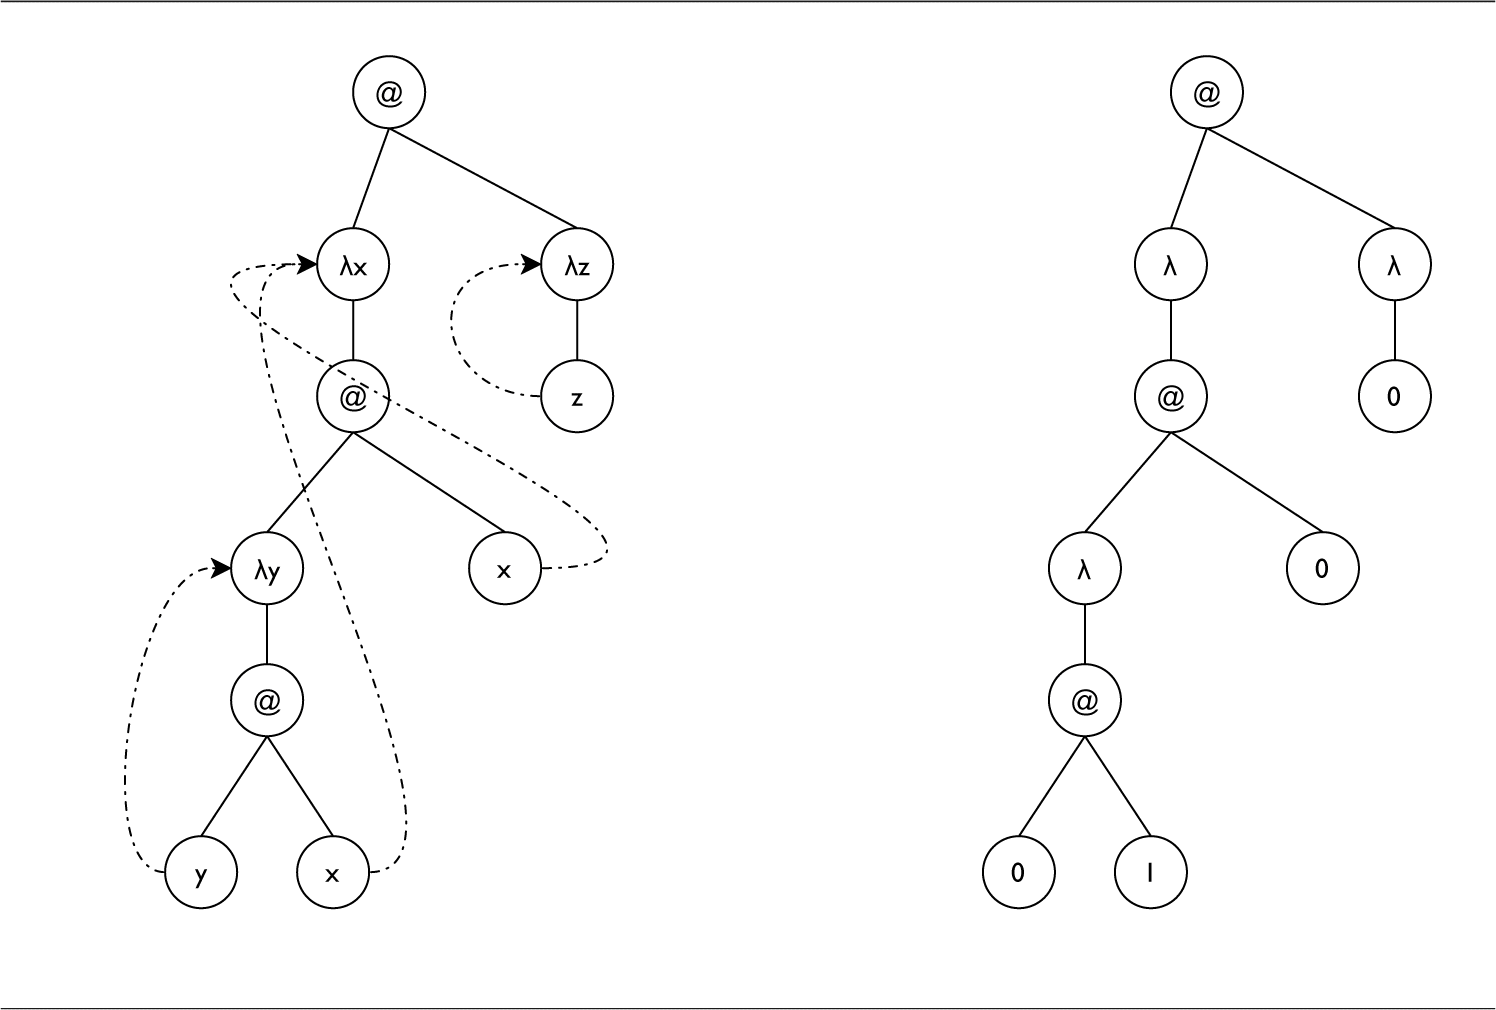
\includegraphics[width=0.85\textwidth]{images/00766.png}
  \caption{静态距离（De Bruijn 索引）与无名抽象语法树}
  \label{fig:188}
\end{figure}

\section{具有累加器的数据表示}
\label{sec:ch32_2_data}

插曲 5 末尾曾指出：*SL 语言在计算列表等容器的大小时，需要从头到尾遍历整个列表，消耗 $\mathcal{O}(n)$ 的时间；而很多现代工业级编程语言采用了一种成本更低的方式来获取大小。本节将展示如何通过\textbf{在数据结构本身中内置累加器}（即\term{数据累加器}，Data Accumulator）来实现这一思想。

回顾第 8.2 节：在 BSL 中，完全可以使用结构体与函数自定义实现一套列表机制，如图 \ref{fig:189} 所示。

\begin{figure}[htbp]
  \centering
\begin{lstlisting}[language=BSL, basicstyle=\scriptsize\ttfamily]
(define-struct pair [left right])
; ConsOrEmpty is one of:
; -- '()
; -- (make-pair Any ConsOrEmpty)

; Any ConsOrEmpty -> ConsOrEmpty
(define (our-cons a-value a-list)
  (cond
    [(empty? a-list) (make-pair a-value a-list)]
    [(our-cons? a-list) (make-pair a-value a-list)]
    [else (error "our-cons: ...")]))

; ConsOrEmpty -> Any
; extracts the left part of the given pair
(define (our-first mimicked-list)
  (if (empty? mimicked-list)
      (error "our-first: ...")
      (pair-left mimicked-list)))
\end{lstlisting}
  \caption{在 BSL 中基于结构体自定义实现的列表机制}
  \label{fig:189}
\end{figure}

实现常数时间获取大小的关键洞见在于：为 \code{pair} 结构体增设第三个字段 \code{count}：

\begin{lstlisting}[language=BSL]
(define-struct cpair [count left right])
; A [MyList X] is one of:
; -- '()
; -- (make-cpair N X [MyList X])
; 累加器说明：count 字段记录构建该列表所包含的 cpair 节点总数
\end{lstlisting}

这里，结构体字段 \code{count} 记录了列表构建过程中的一项累积事实。我们称这种字段为\term{数据累加器}。

当然，天下没有免费的午餐。引入数据累加器必然带来工程权衡：
\begin{enumerate}
  \item \textbf{内存开销}：每个列表节点多占用一个字段，列表的内存占用增加了 33\%；
  \item \textbf{构建开销}：构造函数 \code{our-cons} 在每次添加元素时，都必须额外执行一次累加计算：
\begin{lstlisting}[language=BSL]
(define (our-cons f r)
  (cond
    [(empty? r) (make-cpair 1 f r)]
    [(cpair? r) (make-cpair (+ (cpair-count r) 1) f r)]
    [else (error "our-cons: ...")]))
\end{lstlisting}
  \item \textbf{巨大回报}：求列表长度函数 \code{our-length} 彻底摆脱了 $\mathcal{O}(n)$ 的线性遍历，直接在 $\mathcal{O}(1)$ 常数时间内返回 \code{(cpair-count l)}！
\end{enumerate}

\begin{exercise}{论证 our-cons 的常数时间开销}{518}
论证无论输入列表的长度有多大，\code{our-cons} 的运行耗时始终为严格的常数时间 $\mathcal{O}(1)$。
\end{exercise}

\begin{exercise}{通用列表设计中的权衡探讨}{519}
在通用的系统设计中，为了让 \code{length} 成为常数时间操作，而要求每一次调用 \code{cons} 都承担额外的空间与计算开销，这种权衡是否普遍可接受？请结合本书中对 \code{cons} 的大量使用场景进行反思。
\end{exercise}

\subsection{高级案例：博弈树与“传教士与食人族”谜题}

在许多复杂搜索与人工智能应用中，数据累加器绝非锦上添花的优化，而是求解问题必不可少的关键工具。考查著名的经典智力谜题：

\begin{notebox}[问题陈述：传教士与食人族谜题 (Missionaries and Cannibals)]
3 名传教士和 3 名食人族一同来到一条湍急的大河边。河上只有一条双人划艇，且必须至少有一人划船才能渡河。两岸的任何一处，只要食人族的人数超过传教士的人数，食人族就会吃掉传教士。

请设计一个程序，为他们规划出一条安全的渡河方案，使得所有 6 人最终都能安全抵达右岸，且在任何中间状态下两岸的传教士都不会被吃掉。
\end{notebox}

图 \ref{fig:mc_states} 展示了谜题的状态表示方法：三栏方框分别代表左岸人员、河道与船只位置、右岸人员。黑圈表示传教士，白圈表示食人族。

\begin{figure}[htbp]
  \centering
  
\includegraphics[width=0.55\textwidth]{images/00768.png}\\[1ex]
  
\includegraphics[width=0.75\textwidth]{images/00769.png}
  \caption{传教士与食人族谜题的状态表示图解（初始状态、终局状态与中间状态）}
  \label{fig:mc_states}
\end{figure}

图 \ref{fig:190} 展现了由此派生出的\term{博弈树}（Game Tree）。在每个状态下，根据船上人员的不同组合（最多载 2 人，至少 1 人），生成所有可能的后继状态。

\begin{figure}[htbp]
  \centering
  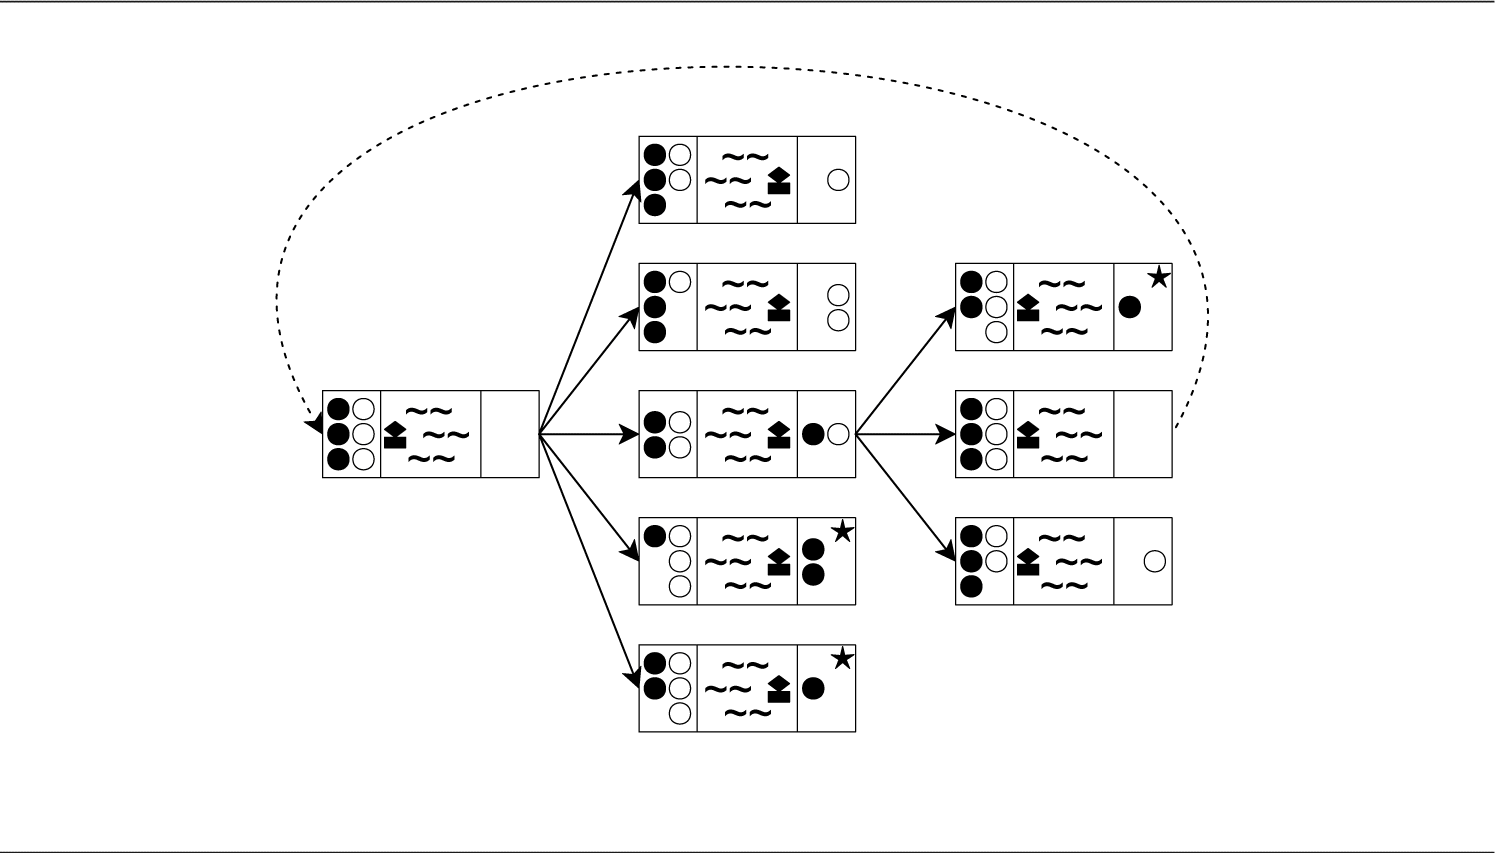
\includegraphics[width=0.85\textwidth]{images/00770.png}
  \caption{传教士与食人族谜题的博弈树推演}
  \label{fig:190}
\end{figure}

仔细观察图 \ref{fig:190} 会发现朴素树搜索面临两个致命挑战：
\begin{enumerate}
  \item \textbf{危险分支（食人状态）}：图中带有星号的分支两岸存在食人族多于传教士的危险状态，必须被剪除；
  \item \textbf{回路死循环（虚线箭头）}：把刚渡过河的人再原样划回来会导致状态复原，从而引发无限搜索循环。
\end{enumerate}

更为根本的是：即使搜索算法找到了终局状态，若仅仅返回最终的那个状态对象，玩家依然一无所获——\textbf{因为算法丢失了“究竟通过怎样的渡河顺序才能从初始状态一步步走到终局”的历史轨迹！}

此时，我们必须在每个状态结构体内部植入一个\term{数据累加器}，用于记录到达当前状态所经历的\textbf{历史状态路径列表}。

\begin{exercise}{广度优先搜索的终止性证明}{520}
原书 \code{solve*} 函数采用逐层探索的广度优先搜索（Breadth-First Search, BFS）策略。论证为何在有限状态空间下，广度优先搜索能够确保找到最短解且不会因为无限递归而遗漏终局。
\end{exercise}

\begin{exercise}{设计谜题状态的数据表示}{521}
为传教士与食人族谜题设计结构体数据定义 \code{PuzzleState}，记录左岸人数、右岸人数以及船的位置。编写判定终局的谓词 \code{final?} 以及图形渲染函数 \code{render-mc}。
\end{exercise}

\begin{exercise}{在状态中植入历史轨迹数据累加器}{522}
修改 \code{PuzzleState} 的结构体定义，为其增设一个数据累加器字段 \code{history}（类型为 \code{[List-of PuzzleState]}），用以记录抵达该状态的历史步骤序列。写出该累加器字段的不变量说明。
\end{exercise}

\begin{exercise}{后继状态生成与危险/循环状态剪枝}{523}
设计后继状态生成函数 \code{create-next-states}。该函数接收当前状态列表，生成一趟合法船行所能达到的所有后继状态列表。利用状态内的数据累加器 \code{history}，过滤掉已访问过的重复状态，并严格剔除传教士会被吃掉的危险状态。
\end{exercise}

\begin{exercise}{输出完整解题路径与动画播放}{524}
完成最终的求解函数 \code{solve}。该函数最终输出从起点到终点的完整状态演化列表，并借助 2htdp/image 与 2htdp/universe 库中的 \code{run-movie} 将渡河解题过程渲染为生动的连续动画！
\end{exercise}

\section{累加器作为计算结果}
\label{sec:ch33_3}

在之前的案例中，累加器主要作为辅助参数用来向递归深处传递上下文信息。而在本节的图形学生成型递归中，我们将见识到累加器的一种更为精妙的全新角色：\textbf{累加器同时作为函数的输入实参、收集绘制图形的载体，以及最终的返回值}！

考虑谢尔宾斯基三角形（Sierpinski triangle）的绘制过程。经典的生成式思想是：若三角形边长足够大，则求出三条边的中点，并对分割出的三个外角小三角形递归进行绘制。

很多程序员直觉上认为可以对三个递归调用分别产生的局部图像调用 \code{overlay} 或 \code{underlay} 组合起来。然而在 DrRacket 交互窗口中的实验无情地打破了这一设想：图库中的图像叠加函数拥有不透明边界，直接叠加会导致后画的图形将先画的三角形遮挡冲刷掉！

\begin{figure}[htbp]
  \centering
\begin{lstlisting}[language=BSL, basicstyle=\scriptsize\ttfamily]
; Image Posn Posn Posn -> Image
; generative adds the triangle (a, b, c) to s,
; subdivides it into three triangles by taking the
; midpoints of its sides; stop if (a, b, c) is too small
(define (add-sierpinski scene0 a b c)
  (cond
    [(too-small? a b c) scene0]
    [else
      (local
        ((define scene1 (add-triangle scene0 a b c))
         (define mid-a-b (mid-point a b))
         (define mid-b-c (mid-point b c))
         (define mid-c-a (mid-point c a))
         (define scene2
           (add-sierpinski scene0 a mid-a-b mid-c-a))
         (define scene3
           (add-sierpinski scene0 b mid-b-c mid-a-b))
         (define scene4
           (add-sierpinski scene0 c mid-c-a mid-b-c)))
        ; ---IN---
        (... scene1 ... scene2 ... scene3 ...))]))
\end{lstlisting}
  \caption{作为生成型递归结果的累加器骨架设计}
  \label{fig:191}
\end{figure}

正确的解题之道在于：\textbf{将底色画布作为累加器在递归调用之间依次串联流转}！
\begin{enumerate}
  \item 首先在原始画布 \code{scene} 上添加第一个三角形，得到更新后的画布 \code{scene1}；
  \item 将 \code{scene1} 作为累加器输入传入第二个递归调用，在它的基础上绘制第二个三角形，得到进一步富化的画布 \code{scene2}；
  \item 将 \code{scene2} 传入第三个递归调用，绘制得到最终完整的画布 \code{scene3} 并将其作为结果返回！
\end{enumerate}

图 \ref{fig:192} 给出了基于这一突破性洞见的完整函数实现。

\begin{figure}[htbp]
  \centering
\begin{stepperbox}[unbreakable]
\begin{Verbatim}[commandchars=\\\{\}, fontsize=\scriptsize]
; Image Posn Posn Posn -> Image
; generative adds the triangle (a, b, c) to s,
; subdivides it into three triangles by taking the
; midpoints of its sides; stop if (a, b, c) is too small
; accumulator the function accumulates the triangles scene0
(define (add-sierpinski scene0 a b c)
  (cond
    [(too-small? a b c) scene0]
    [else
      (local
        ((define scene1 (add-triangle scene0 a b c))
         (define mid-a-b (mid-point a b))
         (define mid-b-c (mid-point b c))
         (define mid-c-a (mid-point c a))
         (define scene2
           (add-sierpinski \hl{scene1} a mid-a-b mid-c-a))
         (define scene3
           (add-sierpinski \hl{scene2} b mid-b-c mid-a-b)))
        ; ---IN---
        (add-sierpinski \hl{scene3} c mid-c-a mid-b-c))]))
\end{Verbatim}
\end{stepperbox}
  \caption{累加器作为计算结果的生成型递归函数实现}
  \label{fig:192}
\end{figure}

\begin{exercise}{实现心愿单几何计算辅助函数}{525}
根据骨架要求，设计三个几何辅助函数：
\begin{enumerate}
  \item \code{add-triangle}：向指定场景中添加由三顶点围成的三角形；
  \item \code{too-small?}：根据两点间欧几里得距离公式判定三角形是否已小于递归阈值；
  \item \code{mid-point}：根据两点中点公式计算线段中点坐标。
\end{enumerate}
\end{exercise}

\begin{exercise}{基于三角函数计算等边三角形顶点 circle-pt}{526}
设计函数 \code{circle-pt}。利用三角函数或极坐标复数运算，计算等边三角形在屏幕坐标系中的三个顶点坐标。注意计算机屏幕坐标系的纵轴正方向朝下。
\end{exercise}

\begin{exercise}{绘制分形萨凡纳树 (Fractal Savannah Tree)}{527}
观察下图（左图展示了一棵优美的分形萨凡纳树，右图解释了其生成式分支步骤）：
\begin{center}
  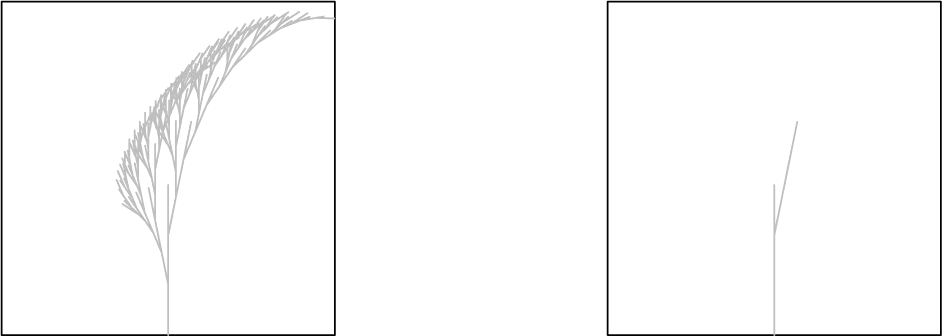
\includegraphics[width=0.65\textwidth]{images/00781.png}

  {\small\textbf{图示：分形萨凡纳树及其几何生成步骤}}
\end{center}
设计函数 \code{add-savannah}，将基底主干三等分，以两个内分点为新起点递归生长左右子枝，并利用画布累加器完成整棵分形树的渲染。
\end{exercise}

\begin{exercise}{生成式绘制贝塞尔光滑曲线 (Bézier Curves)}{528}
计算机图形学中普遍使用贝塞尔曲线连接控制点。下图展示了由德卡斯特里奥（de Casteljau）算法通过连续取中点生成平滑曲线的精妙思想：
\begin{center}
  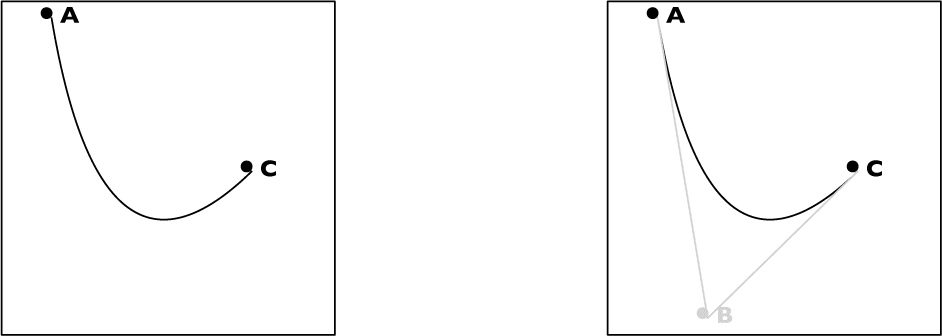
\includegraphics[width=0.45\textwidth]{images/00782.png}\quad
  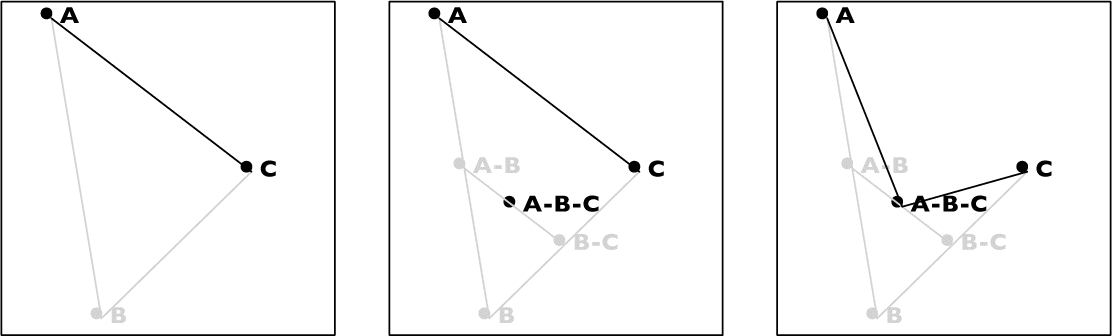
\includegraphics[width=0.45\textwidth]{images/00783.png}

  {\small\textbf{图示：贝塞尔平滑曲线与德卡斯特里奥生成式中点剖分算法}}
\end{center}
运用本节介绍的画布累加器思想，设计生成型递归函数绘制光滑平顺的贝塞尔二次与三次曲线！
\end{exercise}
